% !TeX spellcheck = en_GB

\documentclass[aspectratio=169,handout]{beamer}

\usepackage[utf8]{inputenc}
\usepackage[english]{babel}
%\usepackage{appendixnumberbeamer}

\usepackage{tikz}
\usetikzlibrary{shapes,arrows,positioning,calc}

\tikzstyle{startstop} = [ellipse, draw, fill=bg, text=structure, text width=3em, text badly centered, inner sep=0pt]
\tikzstyle{block} = [rectangle, draw, fill=bg, text=structure, text width=5em, text centered]
\tikzstyle{decision} = [diamond, aspect=3, draw, fill=bg, text=structure, text width=3em, text badly centered, inner sep=0pt]
\tikzstyle{input} = [trapezium, draw, fill=bg, text=structure, text width=5em, text centered, trapezium right angle=120]
\tikzstyle{output} = [trapezium, draw, fill=bg, text=structure, text width=5em, text centered, trapezium right angle=120]

\tikzstyle{line} = [draw, -latex']

%\usepackage{xcolor}
\usepackage{listings}

\lstdefinestyle{pseudo}{
	backgroundcolor=\color{bg},
	keywordstyle=\color{alert},
	numberstyle=\tiny\color{fg!50},
	numbers=left,
	%commentstyle=\color{mGreen},
	%stringstyle=\color{mPurple},
    mathescape=true,
	basicstyle=\scriptsize,
    keywords={input,output,begin,end,if,then,else,while,do,for,each,return}
	%tabsize=4,
	%breakatwhitespace=false,
	%breaklines=true,
	%captionpos=b,
	%keepspaces=true,
	%numbersep=5pt,
	%showspaces=false,
	%showstringspaces=false,
	%showtabs=false,
	%language=C
}

\usepackage{minted}


\usetheme[titleformat=smallcaps, numbering=fraction, background=light, progressbar=frametitle]{metropolis}

\title{Digital Technology}
\subtitle{RESTful APIs, Plots and recap}

\author{Stefano Cereda\\
stefano.cereda@polimi.it
}
\date{12/05/2020}
\institute[PoliMi]{Politecnico Milano}
\logo{
\includegraphics[width=15mm]{../logopolimi}}

\setbeamercovered{invisible}

\makeindex

\begin{document}
\begin{frame}
    \maketitle
\end{frame}

\begin{frame}{RESTful API}
    A RESTful API is an Application Program Interface (API) which uses HTTP requests to GET, POST, PUT, DELETE and PATCH
    data.

    \pause
    Many websites (e.g., Reddit, Twitter, Facebook, Instagram, Weather Underground, GitHub) make many data available via their APIs.

    You can also use APIs to interact with services like Amazon Web Services (AWS), Prometheus, Alexa, Google Home (and all the
    Google products) and many more.

    \pause
    \texttt{urllib} is the standard Python module to manage HTTP requests.
    However, you should \emph{really} prefer the \texttt{requests} module.
\end{frame}

\begin{frame}{Open Notify}
    \href{http://open-notify.org/}{Open Notify} is an open source project providing simple APIs to get:
    \begin{itemize}
        \item the current number of people in space
        \item the current location of the International Space Station (ISS)
        \item a prediction of overhead passes of the ISS
    \end{itemize}
\end{frame}

\begin{frame}[fragile]{People in Space}
    \url{http://api.open-notify.org/astros.json} is the \emph{endpoint} which you can use to know how many people are
    currently in space.

    Try to open the link with a browser, you will receive a json object as an answer.

    Let's try to get the number of people in space using Python:
    \begin{minted}[autogobble, fontsize=\small]{Python}
        import requests

        response = requests.get("http://api.open-notify.org/astros.json")
        if response.status_code != 200:
            print("There was an error")
        else:
            print("The answer is ", response.content)
    \end{minted}
\end{frame}

\begin{frame}[fragile]{Reading the Json answer}
    The answer we received is a bytes object containing the answer we received.
    From the API documentation, we know that the answer is a JSON object.
    \begin{minted}[autogobble, fontsize=\small]{Python}
        import json

        resp_dict = json.loads(response.content.decode('utf-8'))
        # equivalent
        resp_dict = response.json()

        print("There are {} people in space".format(resp_dict['number']))
        for astro in resp_dict['people']:
            print("{} is on the {}".format(astro['name'], astro['craft']))
    \end{minted}
\end{frame}

\begin{frame}[fragile]{When will the ISS pass over PoliMi?}
    \url{http://api.open-notify.org/iss-pass.json} allows you to know when the ISS will be over a certain location.
    The API requires two input fields: \emph{latitude} and \emph{longitude}. By default it gives you the next 5 passes.

    PoliMi lat/lon are: 45.478156, 9.227080

    \begin{minted}[autogobble, fontsize=\tiny]{Python}
        import requests

        params_dict = {
            'lat': 45.478156,
            'lon': 9.227080
        }
        resp = requests.get("http://api.open-notify.org/iss-pass.json", params=params_dict)
        resp = resp.json()

        print("The ISS will pass over PoliMi at {}".format(resp['response'][0]['risetime']))
    \end{minted}

The ISS will pass over PoliMi at 1588888063
\end{frame}

\begin{frame}[fragile]{Help! I cannot put 1588888063 in my calendar!}
    The pass time is returned as a Unix timestamp (we have already seen them with \texttt{time.time()}), we need to
    convert it to a human readable date.

    \begin{minted}[autogobble, fontsize=\tiny]{Python}
        import datetime
        for iss_pass in resp['response']:
            dt = datetime.datetime.utcfromtimestamp(iss_pass['risetime'])
            print("ISS will pass over PoliMi at {} UTC".format(dt.strftime('%Y-%m-%d %H:%M:%S')))
    \end{minted}

    \begin{minted}[autogobble, fontsize=\small]{Text}
    ISS will pass over PoliMi at 2020-05-07 21:47:43 UTC
    ISS will pass over PoliMi at 2020-05-07 23:21:15 UTC
    ISS will pass over PoliMi at 2020-05-08 00:57:49 UTC
    ISS will pass over PoliMi at 2020-05-08 02:35:16 UTC
    ISS will pass over PoliMi at 2020-05-08 04:12:26 UTC
    \end{minted}
\end{frame}

\iffalse
\begin{frame}[fragile]{Help! I cannot go at PoliMi right now!}
    If we want to know when the ISS will be over another city, we need to know its latitude and longitude, but we are
    too lazy to search it.

    \href{https://opencagedata.com/api}{OpenCage} provides reverse and forward geocoding via a RESTful API.

    \begin{minted}[autogobble, fontsize=\tiny]{Python}
        import requests

        pd = {'q': "Rome"}
        resp = requests.get("https://api.opencagedata.com/geocode/v1/json", params=pd)

        print(resp.status_code)
    \end{minted}
    We received an error 401, which means we are not authorized to use this API.

    For most of the available APIs you need to register and receive your personal API key, which allows you to use the
    service.
    Once received, you can just place it in the parameters dictionary using key 'key'.
\end{frame}

\begin{frame}[fragile]{The final program}
    \begin{minted}[autogobble, fontsize=\tiny]{Python}
        import requests
        import datetime

        city = input("Where are you? ")
        pd = {'q': city, 'key' = "YOUR_KEY_HERE"}
        resp = requests.get("https://api.opencagedata.com/geocode/v1/json", params=pd)
        match = resp.json()['results'][0]

        lat = match['geometry']['lat']
        lon = match['geometry']['lng']
        full_name = match['formatted']
        flag = match['annotations']['flag']

        pd = {'lat': lat, 'lon': lon}
        resp = requests.get("http://api.open-notify.org/iss-pass.json", params=pd)
        resp = resp.json()
        print("The ISS will pass over {} {} at:".format(full_name, flag))
        for iss_pass in resp['response']:
            dt = datetime.datetime.utcfromtimestamp(iss_pass['risetime'])
            print(dt.strftime('%Y-%m-%d %H:%M:%S'))
    \end{minted}
\end{frame}
\begin{frame}{The result}
Where are you? Port of Spain\\
The ISS will pass over Port of Spain, Trinidad and Tobago at:\\
2020-05-08 00:41:39\\
2020-05-08 02:16:25\\
2020-05-08 12:11:23\\
2020-05-08 13:49:09\\
2020-05-08 23:56:58
\end{frame}
\fi

\begin{frame}{Further extensions}
    Help! I don't know where I live! \pause \url{https://ip-api.com/}

    Help! I want to know whether the sky will be clear during next pass! \pause \url{https://openweathermap.org/api}

    Help! I want to check whether I am free during next pass and create an event in my calendar! \pause
    \url{https://developers.google.com/calendar}

    \pause
    You can check when is the next pass with clear sky, open your curtains before the
    pass, point your telescope, take a picture, post it on instagram, check the likes you received and have Alexa
    congratulate with you while you drink your automatically brewed coffee.
\end{frame}

\begin{frame}{Matplotlib}
    Matplotlib is a comprehensive library for creating static, animated, and interactive visualizations in Python.

    \pause
    The most used module of Matplotlib is PyPlot, which makes Matplotlib work like MATLAB.
    Each pyplot function makes some change to a figure, and various states are preserved across function calls, so that
    it keeps track of things like the current figure and plotting area. (=> Not a RESTful API)
\end{frame}

\begin{frame}[fragile]{A simple example --- plotting y values}
    \begin{minipage}{0.49\textwidth}
        \begin{minted}[autogobble, fontsize=\small]{Python}
            import matplotlib.pyplot as plt
            plt.plot([1,2,1,2])
            plt.ylabel("Some numbers")
            plt.show()
        \end{minted}
    \end{minipage}
    \pause
    \begin{minipage}{0.49\textwidth}
        \centering
        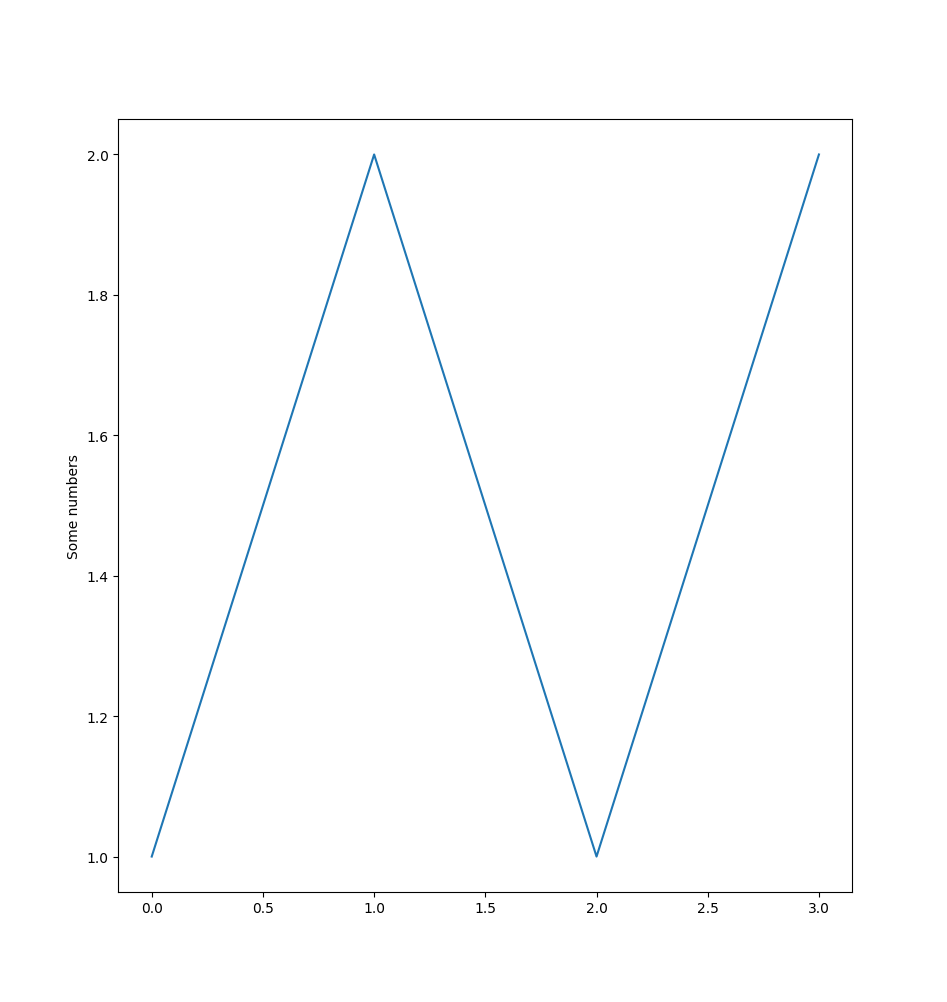
\includegraphics[width=.8\textwidth]{./plots/plot1.png}
    \end{minipage}

    If you provide a single list or array to the plot() command, matplotlib assumes it is a sequence of y values, and
    automatically generates the x values for you.
\end{frame}

\begin{frame}[fragile]{A simple example --- plotting x and y values}
    \begin{minipage}{0.49\textwidth}
        \begin{minted}[autogobble, fontsize=\small]{Python}
            import matplotlib.pyplot as plt
            xs = range(10,100,2)
            ys = [x ** 2 for x in xs]
            plt.plot(xs, ys)
            plt.xlabel("Even numbers")
            plt.ylabel("Squared numbers")
            plt.show()
        \end{minted}
    \end{minipage}
    \pause
    \begin{minipage}{0.49\textwidth}
        \centering
        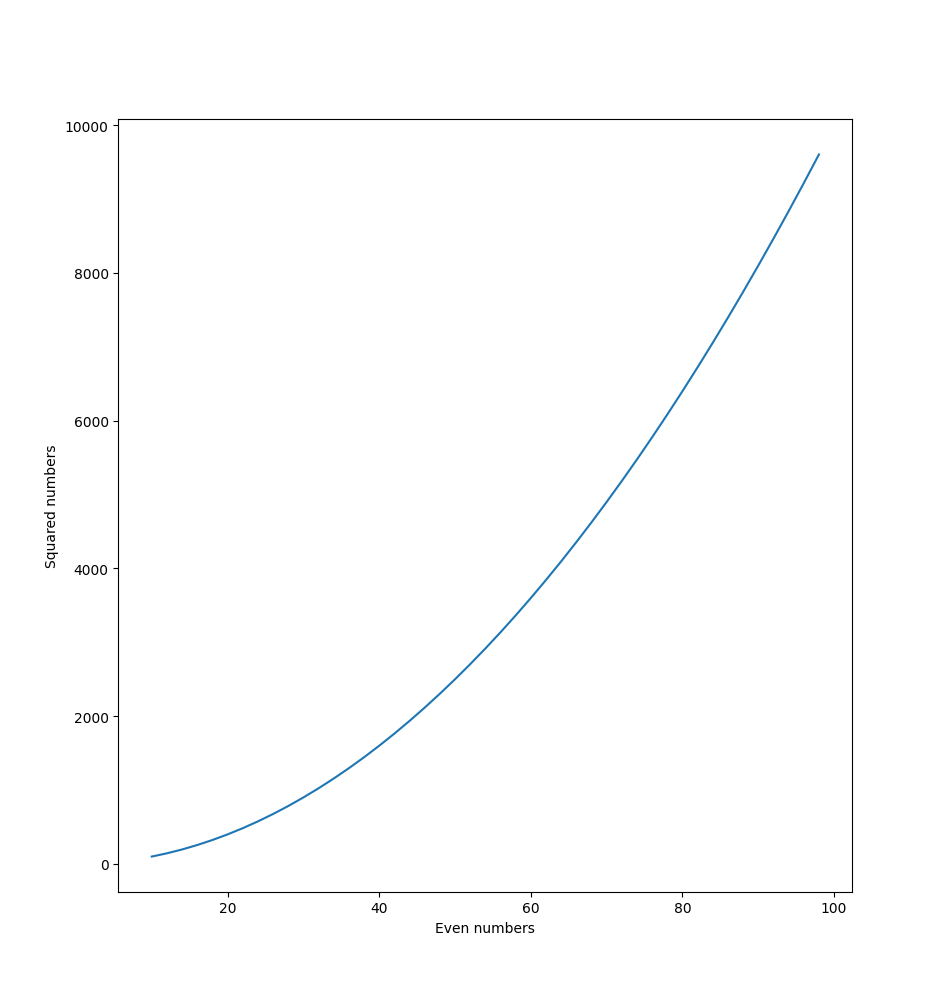
\includegraphics[width=.8\textwidth]{./plots/plot2.png}
    \end{minipage}

    If you give 2 arrays you can plot x versus y (scatter plot).
\end{frame}

\begin{frame}[fragile]{Formatting the style}
    \begin{minipage}{0.49\textwidth}
        \begin{minted}[autogobble, fontsize=\small]{Python}
            import matplotlib.pyplot as plt
            import numpy as np
            xs = np.arange(0, 2*np.pi, 0.001)
            ys_c = np.cos(xs)
            ys_s = np.sin(xs)
            plt.plot(xs, ys_c, 'r--')
            plt.plot(xs, ys_s, 'bo')
            plt.show()
        \end{minted}
    \end{minipage}
    \pause
    \begin{minipage}{0.49\textwidth}
        \centering
        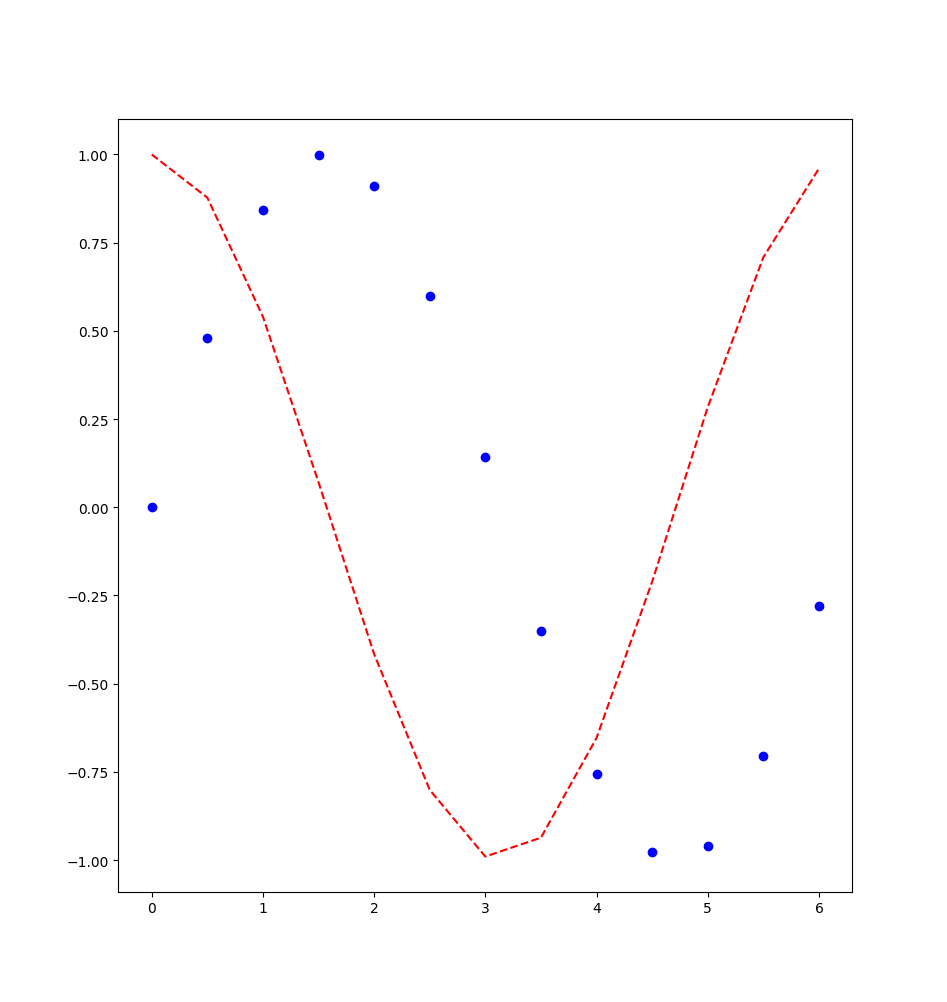
\includegraphics[width=.8\textwidth]{./plots/plot3.png}
    \end{minipage}
    See the \href{https://matplotlib.org/api/_as_gen/matplotlib.pyplot.plot.html#matplotlib.pyplot.plot}{plot()}
    documentation for a complete list of line styles and format strings.
\end{frame}

\begin{frame}[fragile]{Plotting trading strategies}
    We can use this code to get a visualization of our trading strategies:
    \begin{minipage}{0.49\textwidth}
        \begin{minted}[autogobble, fontsize=\tiny]{Python}
import matplotlib.pyplot as plt
import datetime as dt

def plot(days, prices, buys, sells):
    plt.plot(days, prices)
    plt.plot(days[buys], prices[buys], 'go')
    plt.plot(days[sells], prices[sells], 'ro')
    plt.show()

days = stock['Date']
days = [dt.datetime.strptime(d, '%Y-%m-%d').date() for d in days]
days = np.array(days)
plot(days, prices, bk, sk)
plot(days, prices, bg, sg)
        \end{minted}
    \end{minipage}
    \pause
    \begin{minipage}{0.49\textwidth}
        \center
        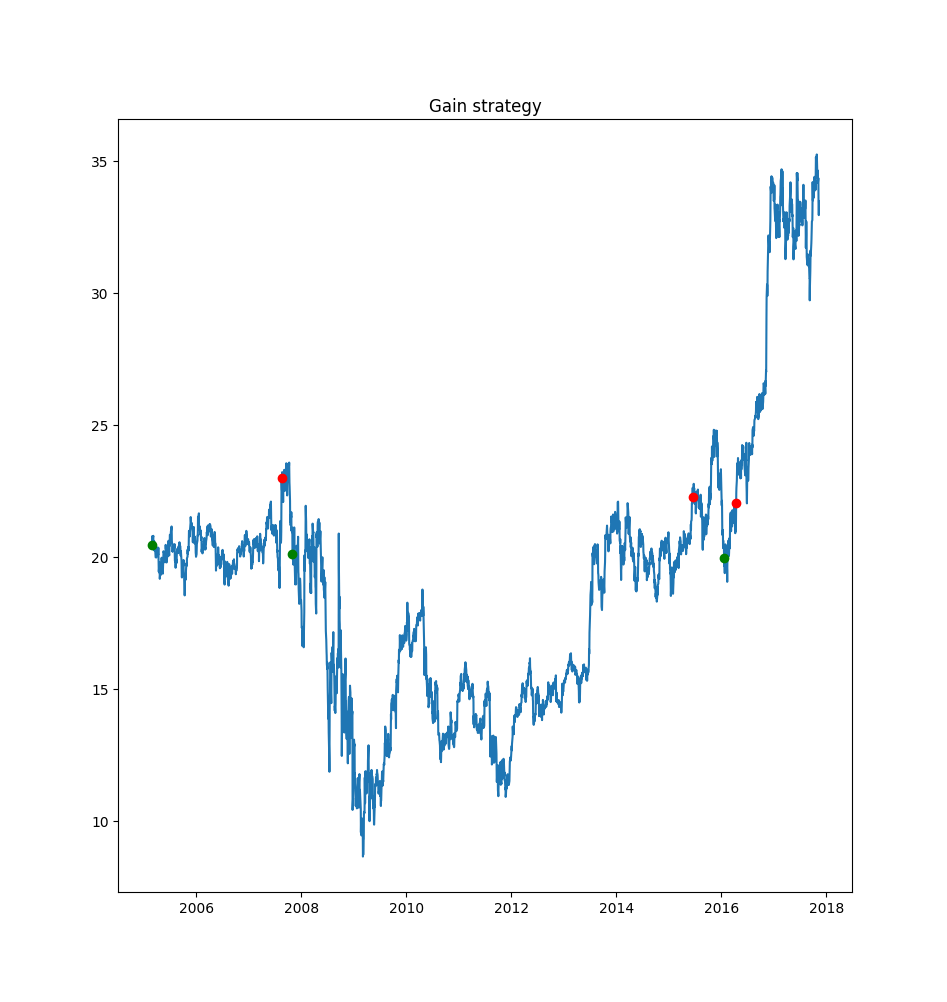
\includegraphics[width=.8\textwidth]{./plots/plot4.png}
    \end{minipage}
\end{frame}

\begin{frame}[fragile]{Multiple plots on the same figure}
    We can plot multiple lines in the same figure:
    \begin{minipage}{0.49\textwidth}
        \begin{minted}[autogobble, fontsize=\tiny]{Python}
            def plot_ma(days, prices, periods):
                plt.plot(days, prices, label='Closing prices')
                for period in periods:
                    ma = moving_average_a(prices, period)
                    plt.plot(days, ma, label='MA period {}'.format(period))
                plt.legend()
                plt.show()

            plot_ma(days, prices, [50,100])
        \end{minted}
    \end{minipage}
    \pause
    \begin{minipage}{0.49\textwidth}
        \begin{flushright}
        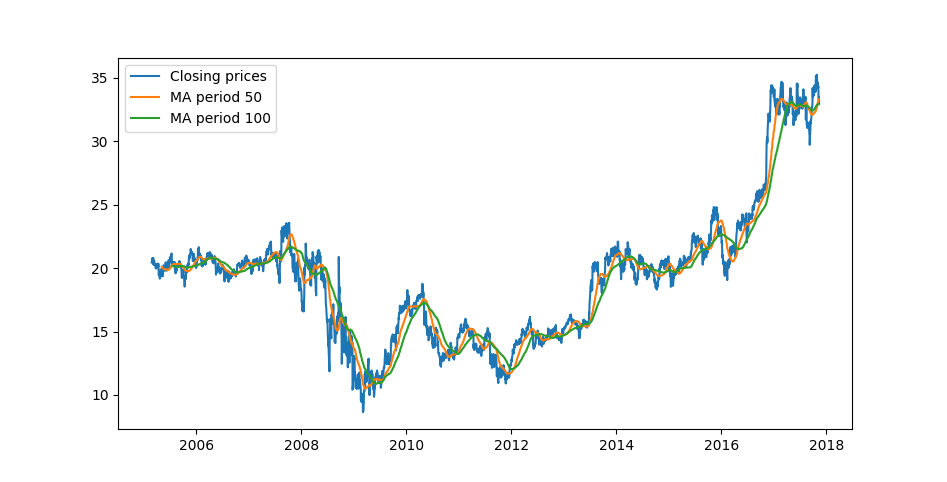
\includegraphics[width=.8\textwidth]{./plots/plot5.png}
        \end{flushright}
    \end{minipage}
\end{frame}

\begin{frame}[fragile]{Plotting the ISS position --- Interactive plots}
    With matplotlib is veary easy to create dynamic plots:
    \begin{minipage}{0.49\textwidth}
        \begin{minted}[autogobble, fontsize=\tiny]{Python}
            import requests
            import time
            import matplotlib.pyplot as plt
            plt.xlim(-180, 180)
            plt.ylim(-90, 90)
            plt.xlabel('Longitude')
            plt.ylabel('Latitude')
            plt.title("ISS position")
            line, = plt.plot([], [], 'bo')
            plt.ion()  # interactive mode
            latitudes = []
            longitudes = []
            while True:
                resp = requests.get("http://api.open-notify.org/iss-now.json")
                if resp.status_code != 200:
                    time.sleep(10)
                    continue
                latitudes.append(float(resp.json()['iss_position']['latitude']))
                longitudes.append(float(resp.json()['iss_position']['longitude']))
                line.set_xdata(longitudes)
                line.set_ydata(latitudes)
                plt.draw()  # force update
                plt.pause(1)  # wait
        \end{minted}
    \end{minipage}
    \pause
    \begin{minipage}{0.49\textwidth}
        \begin{flushright}
        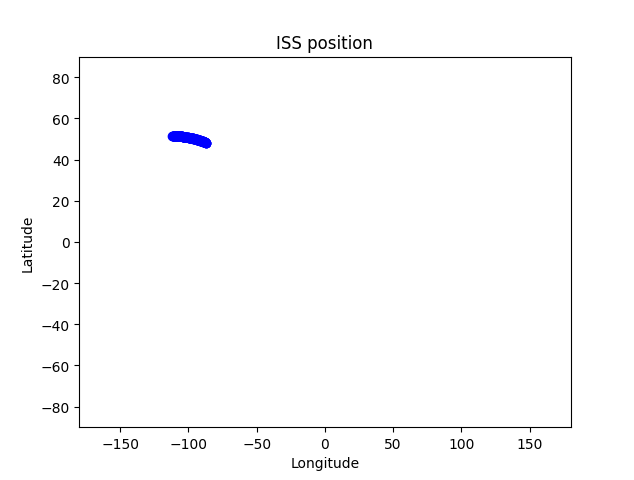
\includegraphics[width=.8\textwidth]{./plots/plot_iss.png}
        \end{flushright}
    \end{minipage}
\end{frame}

\begin{frame}[fragile]{Better geographical plots}
    If you are interested, it's very easy to work with geographical maps:
    \begin{minipage}{0.49\textwidth}
        \begin{minted}[autogobble, fontsize=\tiny]{Python}
            import requests
            import time
            import matplotlib.pyplot as plt
            import mpl_toolkits
            from mpl_toolkits.basemap import Basemap
            plt.ion()  # interactive mode
            m = Basemap(projection='moll', resolution=None, lat_0=0, lon_0=0)
            m.bluemarble(scale=0.5)
            plt.title("ISS position")
            line, = m.plot([], [], 'ro')
            xs = []
            ys = []
            while True:
                resp = requests.get("http://api.open-notify.org/iss-now.json")
                if resp.status_code != 200:
                    time.sleep(10)
                    continue
                lat = float(resp.json()['iss_position']['latitude'])
                lng = float(resp.json()['iss_position']['longitude'])
                x, y = m(lng, lat)
                ys.append(y)
                xs.append(x)
                line.set_xdata(xs)
                line.set_ydata(ys)
                plt.draw()  # force update
                plt.pause(1)  # wait

        \end{minted}
    \end{minipage}
    \pause
    \begin{minipage}{0.49\textwidth}
        \begin{flushright}
        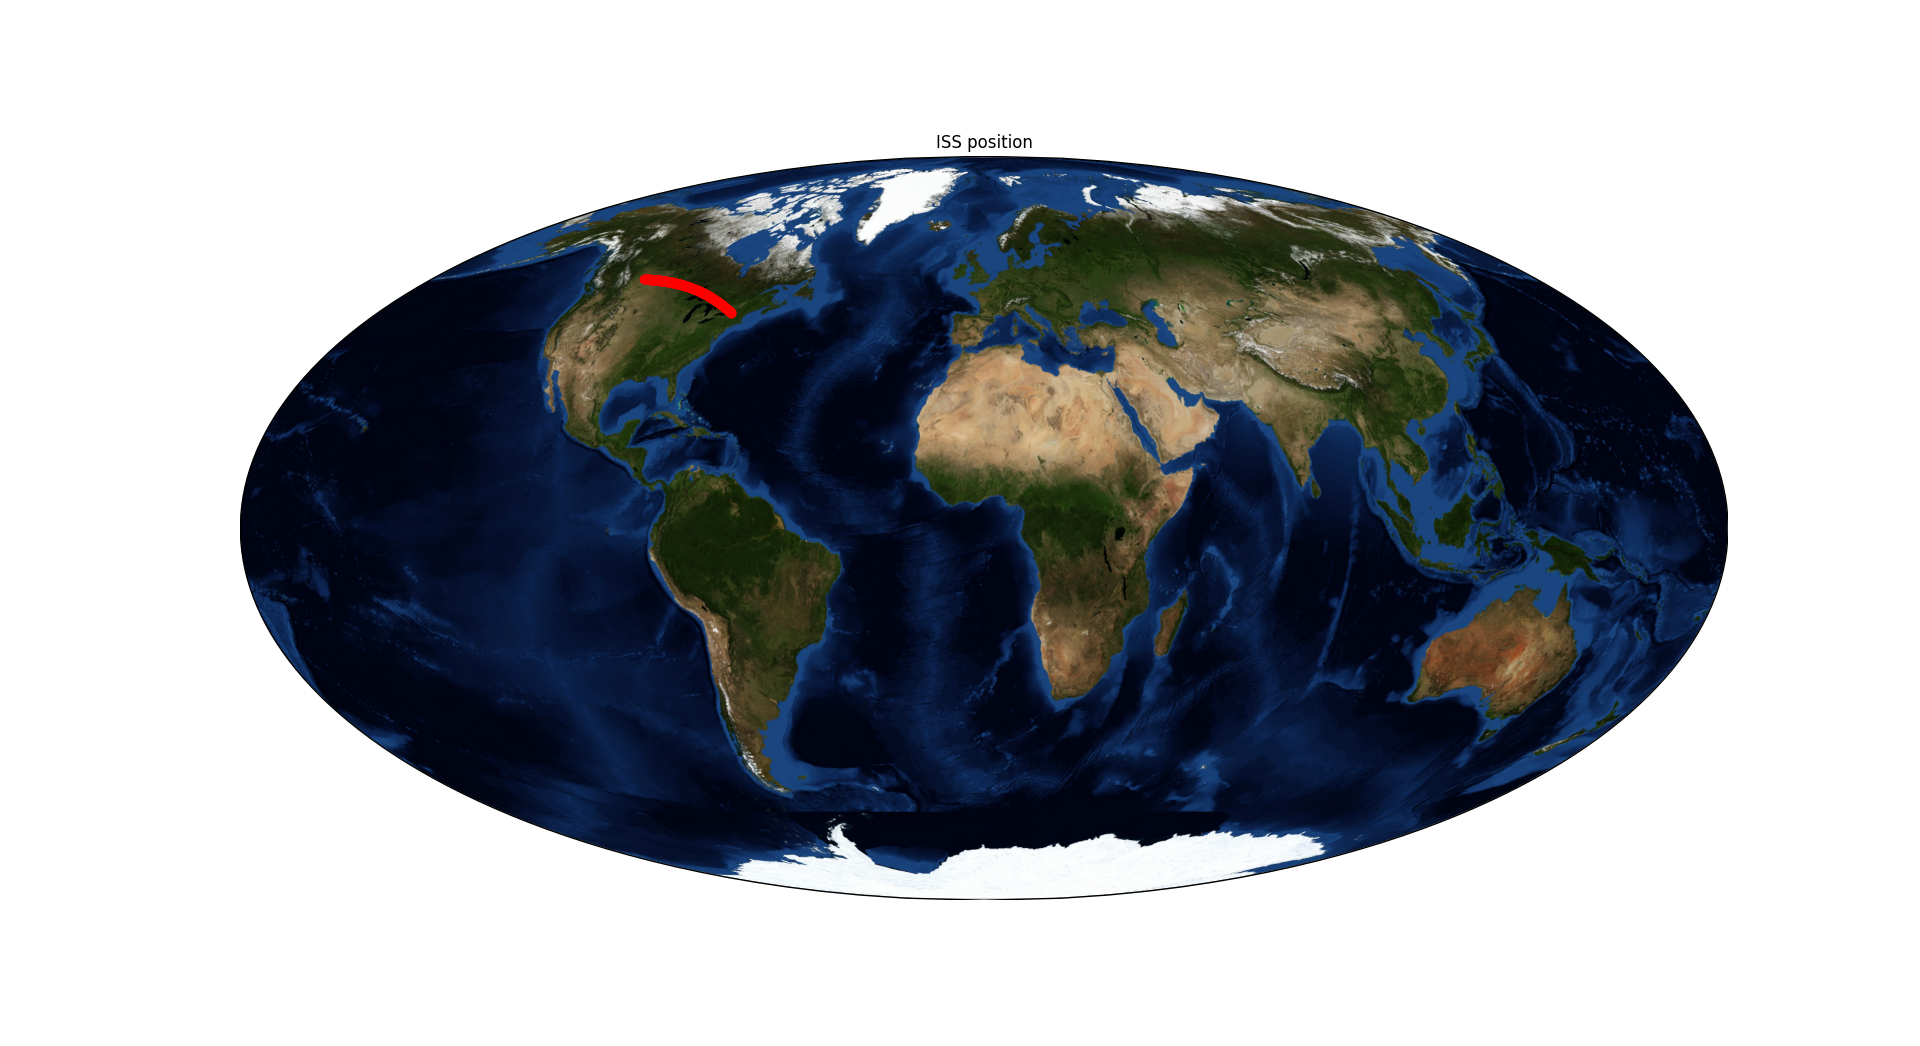
\includegraphics[width=.8\textwidth]{./plots/plot_iss_better.png}
        \end{flushright}
    \end{minipage}
\end{frame}

\begin{frame}[fragile]{Exercise 1 --- Length of words }
    We want to create a list of integers containing the length of each word in a sentence. You can use
    \texttt{sentence.split(char)} to split the string \texttt{sentence} in a list of strings using \texttt{char} as a
    separator.\\
    E.g.: \texttt{"Hello world!".split(' ')} $\rightarrow$ \texttt{["Hello", "world!"]}

    Write a simple piece of Python code using a for loop.

    \pause
    \begin{minted}[autogobble, fontsize=\small]{Python}
        sentence = 'This is an example sentence'
        result = []
        for word in sentence.split(' '):
            result.append(len(word))
        print(result)
    \end{minted}
\end{frame}

\begin{frame}[fragile]{Exercise 2 --- List comprehension}
    Now modify the code to use a list comprehension.

    \pause
    \begin{minted}[autogobble, fontsize=\small]{Python}
        sentence = 'This is an example sentence'
        result = [len(word) for word in sentence.split(' ')]
        print(result)
    \end{minted}
\end{frame}

\begin{frame}[fragile]{Exercise 3 --- Functions}
    Write a function that receives a sentence and returns a list of integers representing the length of each word in a
    sentence except for the word ``the''. Use a list comprehension.

    \pause
    \begin{minted}[autogobble, fontsize=\small]{Python}
        def word_length(sentence):
            return [len(word) for word in sentence.split(' ') if word != 'the']
    \end{minted}
\end{frame}

\begin{frame}[fragile]{Exercise 4 --- Character counter}
    Write a function that receives a string and returns a dictionary representing the number of occurrences of each
    character in the string.

    Solve the exercise using a for loop.

    \pause
    \begin{minted}[autogobble, fontsize=\tiny]{Python}
        def count_char_for1(sentence):
            count = {}
            for character in sentence:
                if character not in count:
                    count[character] = 0
                count[character] += 1
            return count

        def count_char_for2(sentence):
            count = {}
            for character in set(sentence):
                count[character] = sum([c == character for c in sentence])
            return count
    \end{minted}
\end{frame}

\begin{frame}[fragile]{Exercise 5 --- Dictionary comprehension}
    Now solve the exercise using a dictionary comprehension.

    \pause
    \begin{minted}[autogobble, fontsize=\small]{Python}
        def count_char_dc(sentence):
            return {c1: sum([c2 == c1 for c2 in sentence]) for c1 in sentence}
    \end{minted}
\end{frame}

\begin{frame}[fragile]{Exercise 6 --- Simple histograms}
    Use the character counter function to create an histogram of the character occurrences using an asterisk for each
    occurrence.

    You can use print(string, end='') to avoid going to a new line at the end of the print.

    \begin{minipage}{0.49\textwidth}
    \begin{minted}[autogobble, fontsize=\small]{Text}
    E.g. sentence = "Hello world"
    H *
    e *
    l ***
    o **
      *
    w *
    r *
    d *
    \end{minted}
    \end{minipage}
    \pause
    \begin{minipage}{0.49\textwidth}
    \begin{minted}[autogobble, fontsize=\small]{Python}
        count = count_char_dc(sentence)
        for ch in count:
            print(ch, end='')
            for n in range(count[ch]):
                print('*', end='')
            print()
    \end{minted}
    \end{minipage}
\end{frame}

\begin{frame}[fragile]{Exercise 7 --- Simple histograms 2}
    Solve the exercise without using the inner for loop.

    Remember that you can repeat a list using multiplication: \texttt{[1]*4} $\rightarrow$ \texttt{[1,1,1,1]}

    \pause
    \begin{minted}[autogobble, fontsize=\small]{Python}
        count = count_char_dc(sentence)
        for ch in count:
            print(ch, ': ', ['*'] * count[ch])
    \end{minted}
\end{frame}

\begin{frame}[fragile]{Exercise 8 --- Above and below}
    Write a function that receives a list of integers and return two lists: the first one containing the elements above
    the average of the list, the second one containing the elements below.

    Use list comprehension.


    \pause
    \begin{minted}[autogobble, fontsize=\small]{Python}
        def over_under(numbers):
            avg = sum(numbers) / len(numbers)
            above = [num for num in numbers if num > avg]
            below = [num for num in numbers if num < avg]
            return above, below
    \end{minted}
\end{frame}

\begin{frame}[fragile]{Exercise 9 --- Above and below with NumPy arrays}
    Solve the previous exercise using NumPy arrays.

    \pause
    \begin{minted}[autogobble, fontsize=\small]{Python}
        def over_under(numbers):
            avg = np.average(numbers)
            above = numbers[numbers > avg]
            below = numbers[numbers < avg]
            return above, below
    \end{minted}
\end{frame}

\begin{frame}[fragile,allowframebreaks]{Exercise 10 --- Pandas}
    Write a Python program that:
    \begin{enumerate}
        \item Opens the \texttt{aapl.us.txt} csv file
        \item Computes the median value of the ``Open'' column
        \item Creates a new boolean column with title ``above\_median'' containing True in the lines where the 'Close'
            column is above the median of the ``Open'' column.
            \item Saves in a new DataFrame called \texttt{result.csv}
    \end{enumerate}

    You can add a column to a dataframe with: \texttt{my\_df['NewCol'] = values}.

    \framebreak
    \inputminted[autogobble, fontsize=\small]{Python}{./code/pandas_median.py}

\end{frame}
\end{document}
